

% Gradient Info
  
\tikzset {_o27i3u0fi/.code = {\pgfsetadditionalshadetransform{ \pgftransformshift{\pgfpoint{0 bp } { 0 bp }  }  \pgftransformscale{1.8 }  }}}
\pgfdeclareradialshading{_bi11lfu99}{\pgfpoint{0bp}{0bp}}{rgb(0bp)=(1,1,1);
rgb(0bp)=(1,1,1);
rgb(25bp)=(0,0,0);
rgb(400bp)=(0,0,0)}
\tikzset{every picture/.style={line width=0.75pt}} %set default line width to 0.75pt        

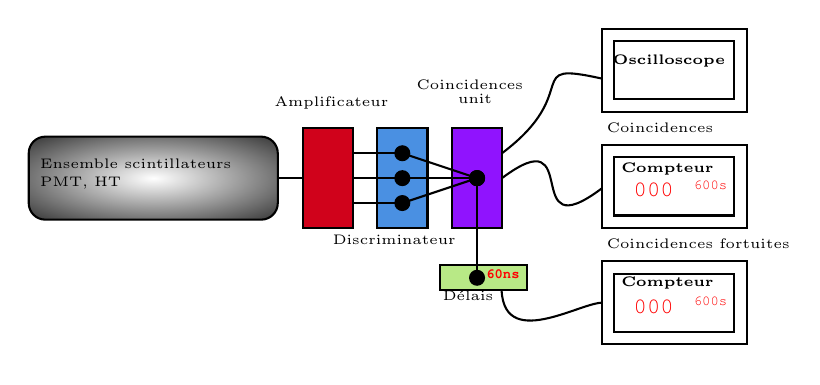
\begin{tikzpicture}[x=0.75pt,y=0.75pt,yscale=-1,xscale=1]
%uncomment if require: \path (0,300); %set diagram left start at 0, and has height of 300

%Shape: Rectangle [id:dp9388352696495245] 
\draw  [fill={rgb, 255:red, 208; green, 2; blue, 27 }  ,fill opacity=1 ] (432,48) -- (456.24,48) -- (456.24,96) -- (432,96) -- cycle ;
%Shape: Frame [id:dp16829955672449592] 
\draw   (576,0) -- (646,0) -- (646,40) -- (576,40) -- cycle(640,6) -- (582,6) -- (582,34) -- (640,34) -- cycle ;
%Shape: Rectangle [id:dp08385564233058351] 
\draw  [fill={rgb, 255:red, 74; green, 144; blue, 226 }  ,fill opacity=1 ] (467.88,48) -- (492.12,48) -- (492.12,96) -- (467.88,96) -- cycle ;
%Shape: Frame [id:dp460543295505199] 
\draw   (576,56) -- (646,56) -- (646,96) -- (576,96) -- cycle(640,62) -- (582,62) -- (582,90) -- (640,90) -- cycle ;
%Curve Lines [id:da19696877411952052] 
\draw    (528,60) .. controls (568,30) and (536.71,15.29) .. (576,24) ;
%Curve Lines [id:da024262443733791716] 
\draw    (528,72) .. controls (568,42) and (536,107) .. (576,77) ;
%Straight Lines [id:da8627449545798643] 
\draw    (456,60) -- (480,60) ;
\draw [shift={(480,60)}, rotate = 0] [color={rgb, 255:red, 0; green, 0; blue, 0 }  ][fill={rgb, 255:red, 0; green, 0; blue, 0 }  ][line width=0.75]      (0, 0) circle [x radius= 3.35, y radius= 3.35]   ;
%Straight Lines [id:da9596413715024262] 
\draw    (456,72) -- (480,72) ;
\draw [shift={(480,72)}, rotate = 0] [color={rgb, 255:red, 0; green, 0; blue, 0 }  ][fill={rgb, 255:red, 0; green, 0; blue, 0 }  ][line width=0.75]      (0, 0) circle [x radius= 3.35, y radius= 3.35]   ;
%Straight Lines [id:da8119306322827472] 
\draw    (456,84) -- (480,84) ;
\draw [shift={(480,84)}, rotate = 0] [color={rgb, 255:red, 0; green, 0; blue, 0 }  ][fill={rgb, 255:red, 0; green, 0; blue, 0 }  ][line width=0.75]      (0, 0) circle [x radius= 3.35, y radius= 3.35]   ;
%Shape: Rectangle [id:dp3987182356264175] 
\draw  [fill={rgb, 255:red, 144; green, 19; blue, 254 }  ,fill opacity=1 ] (503.76,48) -- (528,48) -- (528,96) -- (503.76,96) -- cycle ;
%Straight Lines [id:da6712190365201196] 
\draw    (480,72) -- (516,72) ;
\draw [shift={(516,72)}, rotate = 0] [color={rgb, 255:red, 0; green, 0; blue, 0 }  ][fill={rgb, 255:red, 0; green, 0; blue, 0 }  ][line width=0.75]      (0, 0) circle [x radius= 3.35, y radius= 3.35]   ;
%Straight Lines [id:da780749344939817] 
\draw    (480,84) -- (516,72) ;
\draw [shift={(516,72)}, rotate = 341.57] [color={rgb, 255:red, 0; green, 0; blue, 0 }  ][fill={rgb, 255:red, 0; green, 0; blue, 0 }  ][line width=0.75]      (0, 0) circle [x radius= 3.35, y radius= 3.35]   ;
%Straight Lines [id:da7632950645361253] 
\draw    (480,60) -- (516,72) ;
\draw [shift={(516,72)}, rotate = 18.43] [color={rgb, 255:red, 0; green, 0; blue, 0 }  ][fill={rgb, 255:red, 0; green, 0; blue, 0 }  ][line width=0.75]      (0, 0) circle [x radius= 3.35, y radius= 3.35]   ;
%Curve Lines [id:da7856991642275742] 
\draw    (528,120) .. controls (524.6,157.4) and (563.8,132.6) .. (576,132) ;
%Shape: Rectangle [id:dp7343822070824885] 
\draw  [fill={rgb, 255:red, 184; green, 233; blue, 134 }  ,fill opacity=1 ] (540,114) -- (540,126) -- (498,126) -- (498,114) -- cycle ;
%Straight Lines [id:da9963293912991522] 
\draw    (516,72) -- (516,120) ;
\draw [shift={(516,120)}, rotate = 90] [color={rgb, 255:red, 0; green, 0; blue, 0 }  ][fill={rgb, 255:red, 0; green, 0; blue, 0 }  ][line width=0.75]      (0, 0) circle [x radius= 3.35, y radius= 3.35]   ;
%Shape: Frame [id:dp9715534005025327] 
\draw   (576,112) -- (646,112) -- (646,152) -- (576,152) -- cycle(640,118) -- (582,118) -- (582,146) -- (640,146) -- cycle ;
%Rounded Rect [id:dp0463394923852084] 
\path  [shading=_bi11lfu99,_o27i3u0fi] (300,60) .. controls (300,55.58) and (303.58,52) .. (308,52) -- (412,52) .. controls (416.42,52) and (420,55.58) .. (420,60) -- (420,84) .. controls (420,88.42) and (416.42,92) .. (412,92) -- (308,92) .. controls (303.58,92) and (300,88.42) .. (300,84) -- cycle ; % for fading 
 \draw   (300,60) .. controls (300,55.58) and (303.58,52) .. (308,52) -- (412,52) .. controls (416.42,52) and (420,55.58) .. (420,60) -- (420,84) .. controls (420,88.42) and (416.42,92) .. (412,92) -- (308,92) .. controls (303.58,92) and (300,88.42) .. (300,84) -- cycle ; % for border 

%Straight Lines [id:da13295955815022265] 
\draw    (420,72) -- (432,72) ;

% Text Node
\draw (580,11) node [anchor=north west][inner sep=0.75pt]   [align=left] {{\tiny \textbf{Oscilloscope}}};
% Text Node
\draw (417,31.2) node [anchor=north west][inner sep=0.75pt]   [align=left] {{\tiny Amplificateur}};
% Text Node
\draw (445,98) node [anchor=north west][inner sep=0.75pt]   [align=left] {{\tiny Discriminateur}};
% Text Node
\draw (590,73) node [anchor=north west][inner sep=0.75pt]  [font=\footnotesize] [align=left] {{\fontfamily{pcr}\selectfont {\footnotesize \textcolor[rgb]{1,0,0}{000}}}};
% Text Node
\draw (619,72) node [anchor=north west][inner sep=0.75pt]  [font=\footnotesize] [align=left] {{\fontfamily{pcr}\selectfont {\tiny \textcolor[rgb]{1,0,0}{600s}}}};
% Text Node
\draw (584,63) node [anchor=north west][inner sep=0.75pt]   [align=left] {{\tiny \textbf{Compteur}}};
% Text Node
\draw (485.4,23) node [anchor=north west][inner sep=0.75pt]   [align=left] {{\tiny Coincidences }};
% Text Node
\draw (505.4,30) node [anchor=north west][inner sep=0.75pt]   [align=left] {{\tiny unit}};
% Text Node
\draw (498,125) node [anchor=north west][inner sep=0.75pt]   [align=left] {{\tiny Délais}};
% Text Node
\draw (590,129) node [anchor=north west][inner sep=0.75pt]  [font=\footnotesize] [align=left] {{\fontfamily{pcr}\selectfont {\footnotesize \textcolor[rgb]{1,0,0}{000}}}};
% Text Node
\draw (619,128) node [anchor=north west][inner sep=0.75pt]  [font=\footnotesize] [align=left] {{\fontfamily{pcr}\selectfont {\tiny \textcolor[rgb]{1,0,0}{600s}}}};
% Text Node
\draw (584,118) node [anchor=north west][inner sep=0.75pt]   [align=left] {{\tiny \textbf{Compteur}}};
% Text Node
\draw (577,44) node [anchor=north west][inner sep=0.75pt]   [align=left] {{\tiny Coincidences }};
% Text Node
\draw (577,100) node [anchor=north west][inner sep=0.75pt]   [align=left] {{\tiny Coincidences fortuites}};
% Text Node
\draw (304,61) node [anchor=north west][inner sep=0.75pt]   [align=left] {{\tiny Ensemble scintillateurs}};
% Text Node
\draw (304,70) node [anchor=north west][inner sep=0.75pt]   [align=left] {{\tiny  PMT, HT}};
% Text Node
\draw (519,115) node [anchor=north west][inner sep=0.75pt]  [font=\footnotesize] [align=left] {{\fontfamily{pcr}\selectfont {\tiny \textcolor[rgb]{1,0,0}{\textbf{60ns}}}}};


\end{tikzpicture}
